%
%%%%%%
% 1. use the "modern" or "classic" option to switch between 
% a modern or classic font, respectively.
%
% 2. add/remove the "hyperref" option to enable/disable hyperlinks:
% (remember to remove auxiliary files after adding/removing 
% the "hyperref" option).
%
% 3. add/remove the "printer" option to typeset a printer-friendly 
% (grayscale)/color version of the thesis.
%
% 4. use the "watermark" option to indicate that this is not an actual
% thesis.
%
% 5. use the "histinit" option to enable "historiated initials".
% (If used, all chapter initials declared by the \InitialCharacter{}
% macro are enlarged. If omitted, arguments of \InitialCharacter{}
% are typeset as normal text.)
%
% 6. use the "plain" option to disable tikz graphics in title page
% and part/chapter headers (might help to avoid compilation timeouts).
% Note that "plain" disables CD label and CD cover creation.
%
% 7. use the "noindex" option to (hopefully) avoid compilation timeouts
% when compiling online (disables index generation - note that "\indexGR",
% "\indexEN" invocations need not be removed when toggling this option).
%
% 8. activate the "newlogo" option to use the new official Logo.
%
%%%%%%%%%%%%%%%%%%%%%%%%%%%%%%%%%%%%%%%%%%%%%%%%%%%%%%%%%%%%%%%%%%%%%%%%%%%%%%%
%
% \documentclass[modern,hyperref,watermark,histinit,noindex,plain,newlogo]{ntua-thesis}
\documentclass[modern,hyperref,histinit,noindex,plain,newlogo]{ntua-thesis}
%
%%%%%%%%%%%%%%%%%%%%%%%%%%%%%%%%%%%%%%%%%%%%%%%%%%%%%%%%%%%%%%%%%%%%%%%%%%%%%%%
%
%
%%%%%%%%%%%%%%%%%%%%%%%%%%%%%%%%%%%%%%%%%%%%%%%%%%%%
%% THESIS INFO 
%%%%%%%%%%%%%%%%%%%%%%%%%%%%%%%%%%%%%%%%%%%%%%%%%%%%
%
% ΤΙΤΛΟΣ ΔΙΠΛΩΜΑΤΙΚΗΣ ΕΡΓΑΣΙΑΣ 
%
% Για εξαναγκασμένες αλλαγές γραμμής χρησιμοποιήστε "\\".
% Αν οι αλλαγές γραμμής πρέπει να είναι διαφορετικές στο εξώφυλλο σε σχέση 
% με το εσώφυλλο (σελ. 3), επαναλάβετε τον τίτλο του εξωφύλλου με τις 
% επιθυμητές αλλαγές γραμμής ως προαιρετικό όρισμα της εντολής \title.
%
% Παραδείγματα:
% 1. Όμοιος τίτλος σε εξώφυλλο και εσώφυλλο, με αυτόματες αλλαγές γραμμής:
%	    \title{Πρότυπο Σύστημα Ομότιμων Κόμβων Βασισμένο σε Σχήματα \en{RDF}}
% 2. Όμοιος τίτλος σε εξώφυλλο και εσώφυλλο, με αλλαγή γραμμής μετά τη λέξη
% "Σύστημα":
%	    \title{Πρότυπο Σύστημα \\ Ομότιμων Κόμβων Βασισμένο σε Σχήματα \en{RDF}}
% 3. Διαφορετικές αλλαγές γραμμής σε εξώφυλλο και εσώφυλλο. Στο εξώφυλλο 
% έχουμε αλλαγή γραμμής μετά τη λέξη "Σύστημα", ενώ στο εσώφυλλο η αλλαγή
% γραμμής ακολουθεί τη λέξη "Ομότιμων":
%	    \title[Πρότυπο Σύστημα \\ Ομότιμων Κόμβων Βασισμένο %
%           σε Σχήματα \en{RDF}]% (προαιρετικό όρισμα)
%           {Πρότυπο Σύστημα Ομότιμων \\ Κόμβων Βασισμένο σε %
%           Σχήματα \en{RDF}}% (υποχρεωτικό όρισμα)
%
	\title{Προανάκτηση σε \en{Blockchain Client}\\ με στατική ανάλυση και υποθετική εκτέλεση\\ των Έξυπνων Συμβολαίων}
%%
%
%% -------------------------------------------------------------------
%% ΥΠΟΤΙΤΛΟΣ ΔΙΠΛΩΜΑΤΙΚΗΣ ΕΡΓΑΣΙΑΣ (προαιρετικός)
%
% Αν δεν υπάρχει υπότιτλος, τοποθετήστε τον χαρακτήρα του σχολίου "%"
% πριν από την εντολή \subtitle, ή αφήστε κενό το όρισμα της εντολής.
%
% Παράδειγμα:
%%	\subtitle{Μελέτη και υλοποίηση}
%	\subtitle{Μελέτη και υλοποίηση}
%
%% -------------------------------------------------------------------
%% ΤΟΥ/ΤΗΣ/ΤΩΝ
%
% "του" ή "της" ή "των", ανάλογα με το φύλο/αριθμό του σπουδαστή ή 
% των σπουδαστών
% Παράδειγμα:
%	\toutis{του}
	\toutis{του}
%
%% -------------------------------------------------------------------
%% ΟΝΟΜΑΤΕΠΩΝΥΜΟ ΣΠΟΥΔΑΣΤΗ ΣΤΑ ΕΛΛΗΝΙΚΑ (ΚΕΦΑΛΑΙΑ, ΓΕΝΙΚΗ ΠΤΩΣΗ)
%
% Για περισσότερους του ενός σπουδαστές, διαχωρίστε με ",".
% Παράδειγμα:
%	\authorNameCapitalGR{ΚΩΝΣΤΑΝΤΙΝΟΥ Δ. ΔΗΜΗΤΡΙΟΥ, ΓΕΩΡΓΙΟΥ Π. ΠΑΝΑΓΑΚΗ}
	\authorNameCapitalGR{ΠΑΝΑΓΙΩΤΗ ΓΚΟΝΗ}
%
%% -------------------------------------------------------------------
%% ΟΝΟΜΑΤΕΠΩΝΥΜΟ ΣΠΟΥΔΑΣΤΗ ΣΤΗ ΛΑΤΙΝΙΚΗ ΜΟΡΦΗ (ΠΕΖΑ)
%
% Δηλώστε εδώ τυχόν ονοματεπώνυμα στη λατινική μορφή, αλλιώς αφήστε
% κενό το όρισμα.
% Για περισσότερους του ενός σπουδαστές, διαχωρίστε με ",".
% Παράδειγμα:
%	\authorNameEN{Albert Einstein, George W. Bush} 
	%\authorNameEN{Albert Einstein} 
%
%% -------------------------------------------------------------------
%% ΟΝΟΜΑΤΕΠΩΝΥΜΟ ΣΠΟΥΔΑΣΤΗ ΣΤΑ ΕΛΛΗΝΙΚΑ (ΠΕΖΑ, ΟΝΟΜΑΣΤΙΚΗ ΠΤΩΣΗ)
%
% Για περισσότερους του ενός σπουδαστές, διαχωρίστε με ",".
% Αν τα ονοματεπώνυμα όλων των σπουδαστών είναι σε λατινική μορφή,
% αφήστε κενό το όρισμα.
% Παράδειγμα:
%	\authorNameGR{Κωνσταντίνος Δημητρίου, Γεώργιος Παναγάκης}
	\authorNameGR{Παναγιώτης Γκόνης}
%
%% -------------------------------------------------------------------
%% ΟΝΟΜΑΤΕΠΩΝΥΜΟ ΕΠΙΒΛΕΠΟΝΤΑ ΚΑΘΗΓΗΤΗ
% 
	\supervisor{Νεκτάριος Κοζύρης}
%
%% -------------------------------------------------------------------
%% ΤΙΤΛΟΣ ΕΠΙΒΛΕΠΟΝΤΑ ΚΑΘΗΓΗΤΗ
%
	\supervisorTitle{Καθηγητής Ε.Μ.Π.}
%
%% -------------------------------------------------------------------
%% ΕΠΙΒΛΕΠΩΝ/ΕΠΙΒΛΕΠΟΥΣΑ
%
% "Επιβλέπων" ή "Επιβλέπουσα", ανάλογα με το φύλο του 
% Επιβλέποντα Καθηγητή
	\supervisorMaleFemale{Επιβλέπων}
%
%% -------------------------------------------------------------------
%% ΤΟΠΟΣ/ΜΗΝΑΣ/ΕΤΟΣ ΕΚΔΟΣΗΣ
%
	\thesisPlaceDate{Αθήνα, Μάρτιος 2022}
%
%% -------------------------------------------------------------------
%% ΤΟΠΟΣ/ΜΗΝΑΣ/ΕΤΟΣ ΣΥΓΓΡΑΦΗΣ (Εμφανίζεται στη σελίδα των ευχαριστιών,
%% αν υπάρχει).
%
	\ackPlaceDate{Αθήνα, Μάρτιος 2022}
%
%% -------------------------------------------------------------------
%% ΗΜΕΡΟΜΗΝΙΑ ΕΞΕΤΑΣΗΣ
%
	\examinationDate{????? Μαρτίου 2022}
%% -------------------------------------------------------------------
%% ΗΜΕΡΟΜΗΝΙΑ ΔΗΛΩΣΗΣ ΠΕΡΙ ΜΗ ΛΟΓΟΚΛΟΠΗΣ
%
	\declarationDate{1 Μαρτίου 2022}
%
%% -------------------------------------------------------------------
%% ΕΤΟΣ COPYRIGHT
%
	\copyrightYear{2022}
%
%% -------------------------------------------------------------------
%% ΟΝΟΜΑΤΕΠΩΝΥΜΟ 1ου ΕΞΕΤΑΣΤΗ
%
	\firstExaminer{Γεώργιος Γκούμας}
%
%% -------------------------------------------------------------------
%% ΤΙΤΛΟΣ 1ου ΕΞΕΤΑΣΤΗ
%
	\firstExaminerTitle{Αναπληρωτής Καθηγητής}
%
%% -------------------------------------------------------------------
%% ΟΝΟΜΑΤΕΠΩΝΥΜΟ 2ου ΕΞΕΤΑΣΤΗ
%
	\secondExaminer{Διονύσιος Πνευματικάτος}
%
%% -------------------------------------------------------------------
%% ΤΙΤΛΟΣ 2ου ΕΞΕΤΑΣΤΗ
%
	\secondExaminerTitle{Καθηγητής Ε.Μ.Π.}
%%
%%
%%%%%%%%%%%%%%%%%%%%%%%%%%%%%%%%%%%%%%%%%%%%%%%%%%%%%%%%%%%%%%%%%%%%%%
%% THESIS COLORS: 
%%%%%%%%%%%%%%%%%%%%%%%%%%%%%%%%%%%%%%%%%%%%%%%%%%%%%%%%%%%%%%%%%%%%%%
%%
%% Χρώμα εξωφύλλου - κεφαλαίων
	\chaptercolor{gray!50!brown}
%%
%% Χρώμα παραρτημάτων
	\appendixcolor{brown!60!orange}
%%
%% Χρώμα υπερσυνδέσμων (αν έχει ενεργοποιηθεί η επιλογή "hyperref")
    \hyperlinkcolor{blue}
%%
%% Χρώμα τίτλου εργασίας στο εξώφυλλο (αν δεν έχει ενεργοποιηθεί 
%% η επιλογή "plain")
    \titlecolor{white}
%%
%% Χρώμα υποβάθρου (φόντου) τίτλου εργασίας στο εξώφυλλο (αν δεν έχει 
%% ενεργοποιηθεί η επιλογή "plain")
    \titlebackgroundcolor{gray!60!brown}  
%%
%%
%%%%%%%%%%%%%%%%%%%%%%%%%%%%%%%%%%%%%%%%%%%%%%%%%%%%%%%%%%%%%%%%%%%%%%
%% COVER PAGE IMAGE: 
%%%%%%%%%%%%%%%%%%%%%%%%%%%%%%%%%%%%%%%%%%%%%%%%%%%%%%%%%%%%%%%%%%%%%%
%%
%% Εικόνα εξωφύλλου (προαιρετική)
%% Στην περίπτωση κατά την οποία δεν είναι επιθυμητή η εισαγωγή εικόνας στο εξώφυλλο,
%% διαγράψτε την εντολή \coverpageimage, ή μετατρέψτε την σε σχόλιο (με "%")
%%
%% Σύνταξη:
%%          \coverpageimage{συντελεστής μεγέθυνσης}{όνομα αρχείου εικόνας [πλήρης διαδρομή]}
%%      ή
%%          \coverpageimage[tikz]{συντελεστής μεγέθυνσης}{εντολές TikZ}
%%          (στις εντολές μπορούν να περιλαμβάνονται και δηλώσεις \usetikzlibrary, κ.λπ.)
%%      
%% Παραδείγματα:
%%      - Χρήση εικόνας από το αρχείο "figures/rdf.png" με συντελεστή μεγέθυνσης 0.8:
%%          \coverpageimage{0.8}{figures/rdf.png}
%%      - Χρήση εικόνας TikZ με συντελεστή μεγέθυνσης 0.5:
%%          \coverpageimage[tikz]{0.5}{
%%              \draw[thick, gray] \foreach \x in {18,90,...,306} {
%%                  (\x:4) node{} -- (\x+72:4)
%%                  (\x:4) -- (\x:3) node{}
%%                  (\x:3) -- (\x+15:2) node{}
%%                  (\x:3) -- (\x-15:2) node{}
%%                  (\x+15:2) -- (\x+144-15:2)
%%                  (\x-15:2) -- (\x+144+15:2)
%%              };
%%          }
%%
     %\coverpageimage{0.8}{figures/rdf.png}
%%
%%%%%%%%%%%%%%%%%%%%%%%%%%%%%%%%%%%%%%%%%%%%%%%%%%%%%%%%%%%%%%%%%%%%%%
%
% add custom hyphenation rules here
\hyphenation{ο-ποί-α} 
%
%%%%
%
%
%%%%
% \usepackage[utf8]{inputenc}
% \usepackage[greek,english]{babel}
% \usepackage{alphabeta}
\begin{document}

\beginfrontmatter

\maketitle

	
% Περίληψη
	\begin{abstract}
\selectlanguage{english}
TODO

\begin{keywords}
\selectlanguage{english}
TODO
\end{keywords}

\end{abstract}



\begin{abstracteng}
\selectlanguage{english}
TODO

\begin{keywordseng}
\selectlanguage{english}
TODO
\end{keywordseng}

\end{abstracteng}

% Αφιέρωση
	\thesisDedication{στους γονείς μου}
% Ευχαριστίες
	%%%%%%%%%%%%%%%%%%%%%%%%%%%%%%%%%%%%%%%%%%%%%%%%%%%%%%%%%%%%%%%%%
%%
%% use the starred version of the "acknowledgements" environment
%% to omit signatures from this section, e.g.:
%% \begin{acknowledgements*} ... \end{acknowledgements*}
%% 
%%%%%%%%%%%%%%%%%%%%%%%%%%%%%%%%%%%%%%%%%%%%%%%%%%%%%%%%%%%%%%%%%
\begin{acknowledgements}
TODO
\end{acknowledgements}

% Πίνακας Περιεχομένων
	\tableofcontents
% Κατάλογος Σχημάτων
	\listoffigures
% Κατάλογος Εικόνων
	\listofillustrations
% Κατάλογος Πινάκων
	\listoftables
% Πρόλογος
	\selectlanguage{english}
	\begin{preface}
Στον πρόλογο αναφέρονται θέματα που δεν είναι επιστημονικά ή τεχνικά, όπως το πλαίσιο που διενεργήθηκε η εργασία, ο τόπος διεξαγωγής, το Εργαστήριο στο οποίο εκπονήθηκε κ.λπ. 
\end{preface}
	
\beginmainmatter

%%%%%%%%%%%%%%%%%%%%%%%%%%%%%%%%%%%%%%%%%%%%%%%%%%%%%
%% INCLUDE YOUR CHAPTERS/SECTIONS HERE
%%
% Εισαγωγή
	\markdownInput{../pmd/chap_01.md.md}

% Μέρη/Κεφάλαια
	% \part{Θεωρητικό Μέρος}
	\markdownInput{../pmd/chap_02.md.md}

% \chapter{Θεωρητικό υπόβαθρο}

% \InitialCharacter{Τ}\en{odo}.

% \section{Αλυσίδες κοινοποιήσεων (\en{blockchain})}
% \subsection{Τι είναι τα συστήματα ομότιμων κόμβων}
% Στα μεγάλα κατανεμημένα συστήματα \indexGR{K@κατανεμημένα συστήματα} όπως είναι ο Παγκόσμιος Ιστός, γίνονται εμφανή τα προβλήματα του παραδοσιακού μοντέλου πελάτη/εξυπηρετητή: Οι πηγές πληροφορίας βρίσκονται μαζεμένες σε
% λίγους κόμβους (εξυπηρετητές) στους οποίους συνδέονται πάρα πολλοί
% πελάτες \cite{elli05}.

% Οι αρχές που διέπουν τα συστήματα ομότιμων κόμβων είναι οι εξής:
% \begin{itemize}
% \item Η αρχή του μοιράσματος των πόρων.
% \item Η αρχή της αυτοοργάνωσης.
% \end{itemize}






% \section{Αρχιτεκτονική και υλοποιήσεις για Ethereum} %  λογισμικού (clients)


% \section{Δομή Ethereum}

% \subsection{World state}

% TODO: για τα contracts διαφορά address με code hash
% (χειρόγραφο)

% \subsection{Λογαριασμού (Accounts) και Συμβόλαια (Contracts)}

% Στο Ethereum

% - Accounts
% - Contracts
% - Contract storage

% \subsection{Transaction}
% - transaction
% - to contracts
% - message calls (contract to contract)


% \subsection{Blockchain}
% - txs into blocks
% - mining
% - blocktree, uncles
% - consensus -> blockchain

% \section{Δομές δεδομένων}

% \subsection{Block}

% - body
% % [geth] core/types/block.go:159, == [erigon] core/types/block.go:614
% - header
% % [geth] core/types/block.go:68, == [erigon] core/types/block.go:72

% \subsection{State}

% \subsubsection{Go-ethereum}
% - mMPT
% - state trie (αγνοούμε τα transaction και receipt trie)

% \paragraph{Υλοποίηση}

% Η \lstinline{stateDB} περιέχει τα \lstinline{stateObjects}.
% Τα \lstinline{stateObject} αντιστοιχούν 1 προς 1 σε \lstinline{Account} τα οποία περιγράφουν.
% % [geth] core/state/statedb.go:59-

% Δημιουγούνται διαβάζοντας το αντίστοιχο \lstinline{Account} από τη \lstinline{stateDB}
% % [geth] core/state/statedb.go:489-559

% Εδώ εφαρμόζεται ένα επίπεδο in-memory\footnote{Το επίπεδο αυτό μπορεί να αποθηκευτεί κατά το κλείσιμο του client και στον δίσκο, ώστε να διαβαστεί κατά την εκκίνηση μελλοντικής εκτέλεσης και να μην χρειαστεί να ξανα-δημιουργηθεί.} read-write cache που ονομάζεται (στον κώδικα) \lstinline{snapshot}.
% Έχει πολλαπλά layers τα οποία περιέχουν \lstinline{Accounts} και \lstinline{Storage} που έχουν ήδη διαβαστεί ή τροποποιηθεί κατά την εκτέλεση.
% Η αναζήτηση γίνεται περώντας από τα επίπεδα με τη σειρά, μέχρι να βρεθεί το κλειδί (διεύθυνση \lstinline{Account} ή \lstinline{Storage}) που αναζητήται.
% Αν δεν βρεθεί σε κανένα επίπεδο γίνεται ανάκτηση από το \lstinline{Trie}.
% Λόγο του μεταβλητού και εν δυνάμει μεγάλου πλήθους των layers που πρέπει να εξεταστούν για ένα κλειδί που δεν υπάρχει στο \lstinline{snapshot},
% διατηρείται ένα φίλτρο (filter) Bloom, το οποίο αποφαίνεται για την πιθανή\footnote{
% Σε περίπτωση που το κλειδί υπάρχει, η απάντηση είναι βέβαιη, ενώ σε περίπτωση που δεν υπάρχει, μπορεί να δοθεί ψευδώς θετική απάντηση ότι υπάρχει.
% Αυτή η συμπεριφορά του φίλτρου δεν επιρρεάζει την ορθότητα των αποτελεσμάτων.
% } ύπαρξη ή όχι του κλειδιού σε οποιοδήποτε layer πριν ξεκινήση η αναζήτηση.
% Έτσι, αρκετές άσκοπες αναζητήσεις παρακάμπτωνται.

% Υλοποίηση αναζήτησης (παράδειγμα για \lstinline{Account}):
% % [geth] state/snapshot/difflayer.go:270-350

% Αν αποτύχει:
% % [geth] core/rawdb/accessors_snapshot.go:75-79

% Σε περίπτωση που το \lstinline{snapshot} δεν υπάρχει (πχ δεν έχει δημιουργηθεί ακόμα) ή δεν περιέχει το κλειδί που ζητήται,
% η ανάκτηση γίνεται από το αντίστοιχο \lstinline{state Trie}:
% % [geth] trie/trie.go:113-158

% Η αναζήτηση αυτή πιθανών να προκαλέσει μία ή και παραπάνω αναγνώσεις απ'το δίσκο, με τη διαδικασία αναζήτησης που περιγράψαμε προηγουμένως.
% Η υλοποίση φαίνεται παρακάτω:
% % [geth] trie/trie.go:499-505
% % [geth] trie/database.go:370-404
% % [geth] ethdb/leveldb.go:22,33,61,63,187-194

% Τα \lstinline{stateObject} ανακτούν δεδομένα \lstinline{Storage} με τον ίδιο τρόπο:
% % [geth] core/state/state_object.go:179-265, hil 237,250

% Οι ανακτήσεις δεδομένων \lstinline{Storage} προκαλούνται από εντολές SLOAD/SSTORE κατά την εκτέλεση κάποιου \lstinline{Smart Contract}:
% % [geth] core/vm/instructions.go:516-531

% Επιπλέον ανακτήσεις, αυτή τη φορά για \lstinline{Accounts}, γίνονται κατά την εκτέλεση των transaction καθώς και την ολοκλήρωση της επεξεργασίας ενός \lstinline{Block}:
% % [geth] core/state_processor.go:59,76,88-93, hil 90
% % [geth] consensus/ethash/consensus.go:587-593, hil 592
% % [geth] core/state/statedb.go:823-879, hil 862,864
% % [geth] core/state/statedb.go:450-451,459,463, hil 463

% Τέλος, η εγγραφή όλων των τροποποιήσεων στη βάση στο δίσκο γίνεται αργότερα, με κλήση στο \lstinline{Trie}:
% % [geth] trie/trie.go:517,527,547


% \subsubsection{Erigon}
% - plainstate
% - mutation
% - mdbx
% - hash later

% \paragraph{Υλοποίηση}

% Η οργάνωση της \lstinline{State Database} του \lstinline{Erigon} μοιάζει με αυτή του \lstinline{Go-ethereum}, με αρκετές όμως συμαντικές διαφορές.
% Βλέπουμε και εδώ τα \lstinline{stateObjects} τα οποία όμως περιέχονται στη δομή \lstinline{IntraBlockState}, η οποία επίσης λειτουργεί ως read-write cache.
% Όπως φαίνεται και απ'το όνομά της, έχει ? SCOPE ? εντός ενός block, με την ένοια ότι
% οι τροποποιήσεις κρατώνται στη δομή αυτή μόνο για τη διάρκεια ενός block.
% Θα δούμε αργότερα τι γίνεται κατά την ολοκλήρωση του block.

% Δομή \lstinline{IntraBlockState}:
% % [erigon] core/state/intra_block_state.go:50-85

% Η δημιουργεία του \lstinline{stateObject} γίνεται πάλι με ανάκτηση του αντίστοιχου \lstinline{Account}:
% % [erigon] core/state/intra_block_state.go:553-554,557,559,560,569, hil 569

% Η διαφορά γίνεται εμφανής στην ανάγνωση του \lstinline{Account} μιας και εδώ δεν υπάρχει δομή \lstinline{Trie}:
% % [erigon] core/state/plain_state_reader.go:70,73

% Έτσι φτάνουμε στο επίπεδο της write-back write-cache που ονομάζεται (στον κώδικα) \lstinline{mutation}.
% Αξίζει να σημειωθεί ότι οι αναγνώσεις πρέπει επίσης να κοιτάξουν τη write-cache μιας και μπορεί να έχει γίνει τροποποίηση που δεν έχει αποτυπωθεί ακόμα στην κύρια βάση.

% % [original_erigon] ethdb/olddb/mutation.go:126-135, 186-191, hil 127, 135, 191
% % [original_erigon] ethdb/olddb/mutation.go:75-80
% % [original_erigon] ethdb/olddb/mutation.go:3,13,20-22
% % [erigon_lib]      kv/mdbx/kv_mdbx.go:872-879

% Τα \lstinline{stateObject} ανακτούν δεδομένα \lstinline{Storage} με τον ίδιο τρόπο:
% % [erigon] core/state/state_object.go:159-160,162,174, hil 174
% % [erigon] core/state/state_object.go:184,186,188,211
% % [erigon] core/state/plain_state_reader.go:103,108

% Όπως είδαμε και προηγουμένως, οι ανακτήσεις δεδομένων \lstinline{Storage} προκαλούνται από εντολές SLOAD/SSTORE:
% % [erigon] core/vm/instructions.go:544-562 (remove debug)

% Επίσης, οι ανακτήσεις για \lstinline{Accounts}, που γίνονται κατά την ολοκλήρωση της επεξεργασίας ενός \lstinline{Block}:
% % [erigon] core/blockchain.go:90,123,159,178, hil 178
% % [erigon] core/blockchain.go:248,275,287
% % [erigon] core/state/intra_block_state.go:287-289
% % [erigon] core/state/plain_state_writer.go:125,127

% Εδώ, που πρόκειται να γίνει η οριστικοποίηση του \lstinline{Block}, πρέπει να γίνουν κάποιες εγγραφές.
% Οι εγγραφές αυτές θα καταλήξουν στη write-cache (\lstinline{mutation}) αλλά, μιας και δεν έχουμε τη δομή \lstinline{MPT} (όπως στο \lstinline{go-ethereum}), η διαδικασία διαφέρει αρκετά.
% Η δομή \lstinline{MPT} από μόνη της έχει την ιδιότητα ότι οι εγγραφές δεν πανω-γράφουν (overwrite) τις παλιές τιμές, αλλά,
% χάρη στην συνάρτηση κατακερματισμού\footnote{Τροποποιημένα δεδομένα δίνουν τελείως διαφορετικό αποτέλεσμα κατακερματισμού (\lstinline{hash}) το οποίο χρησιμοποιήται ως νέα διεύθυνση, η οποία είναι άδεια (αγνοώντας συγκρούσεις κατακερματισμού).}, παράγεται νέα (κενή) διεύθυνση στην οποία αποθηκεύονται.
% Αυτό δίνει τη δυνατότητα ιστορικής αναδρομής σε προηγούμενες καταστάσεις (\lstinline{historic states}), απλά αλλάζοντας το \lstinline{root hash}.
% Χωρίς το \lstinline{MPT}, για να έχει ο \lstinline{Erigon} την ίδια δυνατότητα, κρατάει πίνακες στη βάση με τις τροποποιήσεις που έχουν γίνει (\lstinline{change-set}).

% Η ενεργοποίηση είναι προεραιτική και γίνεται στην αρχή της εκτέλεσης:
% % [erigon] eth/stagedsync/stage_execute.go:200,228-232

% Αν ενεργοποιηθεί, οι εγγραφές γίνονται με τον \lstinline{change_set_writer}:
% % [erigon] core/state/change_set_writer:119,120,124,125,133,140,141

% Η συνάρτηση \lstinline{Encode()} κάνει απλή μετάφραση και ταξινόμηση:
% % [erigon] common/changeset/account_changeset.go:23-35
% (υπάρχει και αντίστοιχη για \lstinline{Storage})

% Η συνάρτηση \lstinline{AppendDup()} είναι ισοδύναμη με την \lstinline{Put()} στο \lstinline{mutation} που είδαμε προηγουμένως.
% % [original_erigon] ethdb/olddb/mutation.go:204-206

% \section{EVM}

% \subsection{Μοντέλο εκτέλεσης transaction}

% μοντέλο εισόδου-εξόδου, μνημών, εξαιρέσεων
% μοντέλο επεξεργασίας, αρχιτεκτονική στοίβας

% \subsection{Προγραμματισμός SC σε υψηλό επίπεδο - Solidity}

% βασικά για solidity lang
% έξοδος του compiler (creation, runtime)
% δομή του runtime εκτελέσιμου
% - dispatch - μέθοδοι και κλήσεις
% - 'τακτοποίηση' δεδομένων σε μόνιμη μνήμη του contract






































% % \src{
% % \begin{example}
%   % \caption{Κάποιος αλγόριθμος ...}
%   % \lstset{language=C}
% % \begin{lstlisting}
% \begin{lstlisting}[language=go]
% hello(hello, bb uint64)
% world(aa int)
% for 1 := range aa {
%     do {
%         break;
%     }
% }
% \end{lstlisting}
% % \end{example}
% % }
	\markdownInput{../pmd/chap_03.md.md}

    % \part{Πρακτικό Μέρος} 
	\markdownInput{../pmd/chap_04.md.md}

	\markdownInput{../pmd/chap_05.md.md}

% \chapter{Υλοποίηση συστήματος προανάκτησης}

% Στο κεφάλαιο αυτά περιγράφεται συνοπτικά η αρχιτεκτονική του συστήματος, καθώς και οι στόχοι και περιορισμοί που τέθηκαν για την υλοποίησή του.

% \subsection{Σκοπός και περιορισμοί}

% Όπως περιγράφηκαι στο προηγούμενο κεφάλαιο, η διαδικασία του συγχρονισμού στον client \lstinline{erigon} διεκπεραιώνεται σε διακριτά στάδια.
% Μιας και το στάδιο εκτέλεσης των συναλλαγών (\lstinline{Execution stage}) ? accounts for ? τον περισσότερο χρόνο ολόκληρης της διαδικασίας,
% η συγκεκριμένη εργασία περιορίστηκε στην επιτάχυνση αυτού του σταδίου και μόνο.
% Επομένως, κάθε επιλογή που εξετάζεται αναφέρεται στο συγκεκριμένο στάδιο και τα αποτελέσματα που αναφέρονται στα υπόλοιπα κεφάλαια,
% αγνοούν το χρόνο εκτέλεσης των υπόλοιπων σταδίων, κάποια εκ των οποίων (πχ μεταφόρτωσης του blockchain - \lstinline{Downloading stage})
% θα ήταν ανώφελο να μετρηθούν μιας και εξαρτώνται από συνθήκες δικτύου που ? vary widely ? χρονικά και γεωγραφικά.

% Ο σκοπός της εργασίας είναι η βελτίωση της ταχύτητας αυτού του σταδίου με την παράλληλη προανάκτηση προβλεπόμενων εγγραφών από τη βάση δεδομένων.
% Το σύστημα περιορίζεται σε κοινό και εμπορικά διαθέσιμο υλισμικό (\lstinline{hardware}).
% Επίσης, για να διασφαλιστεί η ασφάλεια της διαδικασίας εκτέλεσης των contract, λόγω της ? high stakes ? φύσης της, οι ενέργειες της προανάκτησης
% δεν θα πρέπει να καθορίζουν τα δεδομένα που χρησιμοποιούνται και αποθηκεύονται στο \lstinline{Wolrd State}.
% Έτσι, τυγχών σφάλματα (bugs) ή αδυναμίες (vulnerabilities) σε αυτό το κομμάτι δεν θα threat to compromise την ασφάλεια ολόκληρου του συστήματος,
% και η εκτέλεση θα μπορεί σε κάθε περίπτωση να προχωρά κανονικά, πιθανών επιρρεασμένη μόνο ως προς το χρόνο εκτέλεσης.
% Σε καμία περίπτωση δεν θα πρέπει το κομμάτι της προανάκτησης να έχει τη δυνατότητα να τροποποιήσει δεδομένα του \lstinline{World State}.
% Αυτό περιορίζει τη δυνατότητα προ-επεξεργασίας δεδομένων που θα μπορούσε να αποφέρει καλύτερες επιδόσεις
% αλλά θα έκανε πιο πολύπλοκη τη λογική του κρίσιμου σταδίου της εκτέλεσης που θα δημιουργούσε περισσότερες θέσεις για πιθανά σφάλματα.
% Μοναδική εξέραιση στα παραπάνω θα αποτελέση η προανάκτηση των block η οποία όμως γίνεται ντετερμινιστικά και χωρίς αλλαγές από τον αρχικό κώδικα,
% παραμόνο η τοποθέτησή της σε ξεχωριστό νήμα (thread).

% Τέλος, σε πιθανή ? fatal ? αποτυχία και διακοπή της διαδικασίας προανάκτησης, η κύρια εκτέλεση του client θα συνεχίζεται σαν να μην υπήρχε εξ'αρχής.

% \subsection{Αναλυτική περιγραφή}

% Η εργασία αποτελείται από 3 συνολικά κομμάτια που θα εξεταστούν παρακάτω:
% \begin{itemize}
% \item Iχνογράφηση (Tracing):     Συλλογή μετρικών και κώδικα των contracts
% \item Ανάλυση:                   Ανάλυση των contracts που συλλέχθηκαν στην ιχνογράφηση και σύνθεση των \lstinline{predictors}
% \item Προανάκτηση (Prefetching): Προανάκτηση και υποθετική εκτέλεση των \lstinline{predictors} που δημιουργήθηκαν στην ανάλυση
% \end{itemize}

% Τα κομμάτια της ιχνογράφησης και ανάλυσης στις δοκιμές του επόμενου κεφαλαίου εκτελούνται ξεχωριστά, για λόγους απλότητας,
% αλλά σε μια πραγματική υλοποίηση αναμένουμε να τρέχουν ταυτόχρονα, παράλληλα με την κύρια εκτέλεση.

% \subsubsection{Tracing}

% Σε αυτό το κομμάτι γίνεται συλλογή δεδομένων κατά την πραγματική εκτέλεση των transaction.

% Πιο συγγεκριμένα, καταγράφονται τα code hashes των contract που εκτελλούνται καθώς και το πλήθος
% των κλήσεων (message call) που γίνονται στο καθένα, σε μια δομή αντιστοίχισης από code hash σε πλήθος κλήσεων.
% \begin{lstlisting}[language=go]
% var CONTRACT_CODE_COUNT = map[Hash]uint{}
% \end{lstlisting}

% Επίσης, δεδομένου ότι το code hash έχει πάνω από ένα προκαθορισμένο όριο κλήσεων, αποθηκεύεται και ο κώδικάς του,
% ο οποίος θα περάσει στον αναλυτή, όπως περιγράφεται στο επόμενο στάδιο \lstinline{Analysis}.
% \begin{lstlisting}[language=go]
% var CONTRACT_CODE       = map[Hash][]byte{}
% \end{lstlisting}

% Τέλος, για κάθε εντολή διακλάδωσης που εκελείται καταγράφεται η διεύθυνση του program counter πριν και μετά την εκτέλεση,
% καθώς και το code hash και ένας μοναδικός αριθμός που αντιστοιχεί στο message call που εκτελείται εκείνη τη στιγμή.
% Αποθηκεύεται το πλήθος αυτών των τετράδων.
% \begin{lstlisting}[language=go]
% // code hash -> source -> destination -> call id -> counter
% var JUMP_DST_CALLCOUNT = map[Hash]map[uint32]map[uint32]map[int]uint{}
% \end{lstlisting}
% Στην μέχρι τώρα υλοποίηση, το πλήθος αυτό αγνοήται και κρατάται μόνο η ύπαρξή του (δηλαδή αν είναι διάφορο του 0),
% ώστε να γίνει καταμέτρηση μόνο ως προς το πλήθος των κλήσεων και όχι των διακλαδώσεων.
% Η καταμέτρηση αφορά το κάθε code hash ξεχωριστά και γίνεται μετά την εκτέλεση για λόγους απλότητας,
% αλλά δεν υπάρχει λόγος για τον οποίο δεν μπορεί να γίνει σε προκαθορισμένα χρονικά διαστήματα ή όταν ξεπεραστεί κάποιο όριο.
% Σκοπός τη καταμέτρησης είναι η συλλογή για κάθε code hash που θα αναλυθεί των συχνών διακλαδώσεων.
% Η συλλογή αυτή είναι προαιρετική αλλά είναι συμαντική για καλά αποτελέσματα στο στάδιο της ανάλυσης,
% οπότε σε όλα τα πειράματα της εργασίας είναι ενεργοποιημένη.
% Ο λόγος που κρατάται προαιρετική είναι για πολύ λίγα contracts στα οποία δεν υπάρχουν πολλές κλήσεις για να εξαχθούν χρήσιμα δεδομένα
% και τα οποία επομένως περνάνε στην ανάλυση χωρίς γνωστές διακλαδώσεις.

% \subsubsection{Analysis}

% Το κομμάτι της ανάλυσης αποτελεί το μεγαλύτερο μέρος αυτής της εργασίας.
% Ο σκοπός του είναι να διαβάζει τον κώδικα (runtime bytecode) των contract καθώς συλλέγονται στο προηγούμενο στάδιο,
% καθώς και (προαιρετικά) τις γνωστές διακλαδώσεις για υποβοήθηση,
% και να παράγει ένα νέο κώδικα για το καθένα, που εδώ ονομάζουμε ? προβλεπτή ? (\lstinline{predictor}).
% Οι \lstinline{predictors} χρησιμοποιούνται στο επόμενο στάδιο για την προανάκτηση των δεδομένων που προβλέπεται ότι θα χρησιμοποιήσει η κάθε κλήση (message call).

% Η ανάλυση γίνεται στατικά\footnote{εκτός από τις γνωστές διακλαδώσεις που αναφέρθηκαν προηγουμένως και θα μπορούσε κανείς να ισχυριστεί ότι πρόκειται και για δυναμική ανάλυση},
% ξεκινώντας με ? disassembly ? του EVM κώδικα που βρίσκεται σε δυαδική αναπαράσταση (\lstinline{bytecode}).
% ΣΧΗΜΑ

% Μετά χωρίζεται σε basic block. Αρκετά χρήσιμη για αυτό το στάδιο είναι η επιβολή της εντολής \lstinline{JUMPDEST} του EVM
% σε όλες τις διευθύνσεις στις οποίες επιτρέπεται να φτάσει η ροή της εκτέλεσης από εντολή άλματος.
% ΣΧΗΜΑ

% Στη συνέχεια, οι εντολές που περιέχουν τα basic block μετατρέπονται σε μορφή Static Single Assignment (\lstinline{SSA}) [ REF ].
% ΣΧΗΜΑ
% Εδώ φαίνεται πως γίνεται και μετατροπή της αρχιτεκτονικού μοντέλου από την αρχιτεκτονική στοίβας του EVM σε άπειρων καταχωριτών του SSA,
% εξαλείφοντας εντολές όπως \lstinline{PUSH}, \lstinline{POP} και \lstinline{SWAP}, ενώ δημιουργούνται νέες πσευδο-εντολές Φ (phi) [ REF ].
% Σε αυτό το σημείο ξεκινάει και η πρώτη υποθετική βελτιστοποίηση (speculative optimization) που κάνουμε με το σημάδεμα (marking) για παράκαμψη (skip) των
% block που περιέχουν εντολές που αυθαίρετα θεωρούμε σπάνιες (\lstinline{CREATE}, \lstinline{CREATE2}, \lstinline{INVALID}, \lstinline{REVERT}, \lstinline{SELFDESTRUCT}).
% Block που έχουν σημειωθεί για παράκαμψη θα αγνοούνται.

% Η διαδικασία συνεχίζει με τη σύνδεση των block για τη δημιουργία μιας πρώτης εικόνας του γράφου ελέγχου ροής (CFG).
% Ας σημειωθεί ότι ο CFG σε αυτό το στάδιο δεν είναι ο πραγματικός αλλά μια εκτίμηση.
% Γενικώς, σε επόμενα βήματα θα γίνονται αλλαγές στην εκτίμηση του CFG για να φτάσει πιο κοντά στον πραγματικό,
% αλλά ο βέβαιος προσδιορισμός του είναι αδύνατος μιας και το EVM είναι αρχιτεκτονική turing complete [YP, απόδειξη σε παράρτημα].
% Εδώ χρησιμοποιείται και η πληροφορία για τις γνωστές διακλαδώσεις (αν υπάρχουν) από το προηγούμενο στάδιο.
% Κατά τη διαδικασία αυτή, οι ψευδο-εντολές Φ αποκτούν και της παραμέτρους (arguement/operand) τους.
% ΣΧΗΜΑ

% Ακολουθεί το βήμα της 'βελτιστοποίησης', το οποίο είναι το μεγαλύτερο χρονικά και από θέμα έκτασης κώδικα,
% το οποίο εκτελεί και άλλες λειτουργίες πέραν της βελτιστοποίησης.
% Χρησιμοποιεί τον αλγόριθμο \lstinline{worklist} [ REF ] για να λύσει, μεταξύ άλλων, τα παρακάτω dataflow προβλήματα [ REF is dataflow analysis ]:
% \begin{itemize}
% \item Αντικατάσταση σταθερών (constant folding) [ REF ]
% \item Αλγεβρική απλοποίηση [ REF ]
% \item Σύνολα πιθανών τιμών [ REF is dataflow analysis ]
% \end{itemize}

% Το τελευταίο χρειάζεται για τον προσδιορισμό των πιθανών τιμών των παραμέτρων των εντολών διακλάδωσης (\lstinline{JUMP}, \lstinline{JUMPI}),
% και συγκεκριμένα των πιθανών διευθύνσεων άλματος, σε περίπτωση που δεν είναι γνωστές, για να γίνουν οι αντίστοιχες τροποποιήσεις στην εκτίμηση του CFG.
% Πέραν αυτών, γίνεται αντικατάσταση και ορισμένων εντολών με σταθερές που είναι ήδη γνωστές, όπως η ταυτότητα αλυσίδας (\lstinline{CHANID}), η τιμή του program counter (\lstinline{PC})
% και δεδομένα σχετικά με τον κώδικα που αναλύεται (\lstinline{CODESIZE}, \lstinline{CODECOPY}).

% Επιπλέον, γίνεται και αναδρομική επέκταση του σημαδέματος των block για παράκαμψη σε αυτά που καταλήγουν αναγκαστικά σε σημαδεμένα block,
% καθώς και εξάλειψη των απρόσιτων block (unreachable code elimination), τα οποίο μπορεί να έχει προκληθεί από τη διαδικασία σημαδέματος.

% ΣΧΗΜΑ

% Η διαδικασία συνεχίζει με την επιλογή των εντολών που χρειάζεται να υπάρχουν στην έξοδο, δηλαδή στους predictors.
% Αυτές είναι εντολές που είτε χρησιμοποιούν τη μνήμη \lstinline{storage} του constact (\lstinline{SLOAD}, \lstinline{SSTORE}),
% είτε προκαλούν νέα message calls (\lstinline{CALL}, \lstinline{CALLCODE}, \lstinline{DELEGATECALL}, \lstinline{STATICCALL}),
% είτε τερματίζουν την κλήση και επιστρέφουν δεδομένα (\lstinline{RETURN}, \lstinline{REVERT}).
% Από αυτές, αγνοήται η εντολή \lstinline{REVERT} που προηγουμένως χαρακτηρίστηκε ως σπάνια και επομένως δεν συμπεριλήφθηκε στην ανάλυση.
% Όπως είναι προφανές, δεν αρκεί μόνο η επιλογή αυτών των εντολών, αλλά χρειάζονται και όλες οι υπόλοιπες από τις οποίες εξαρτώνται,
% καθώς και τα block στα οποία περιλαμβάνονται, με την προσθήκη των απαραίτητων εντολών διακλάδωσης και εξαρτήσεων αυτών.
% Επομένως προκύπτει ένα νέο (backward) dataflow πρόβλημα, το οποίο επιλύεται πάλι με τον αλγόριθμο worklist.
% Μία χρήσιμη παρενέργεια αυτής της διαδικασίας είναι και η εξάλειψη άχρηστου κώδικα (dead code elimination),
% μιας και εντολές που δεν χρησιμοποιούνται (από το πρόγραμμα εξόδου) δεν πρόκειται να επιλεγούν.

% ΣΧΗΜΑ
% (οι επιλεγμένες εντολές έχουν ένα αστεράκι * στα αριστερά των διευθύνσεων, ομοίως και τα επιλεγμένα block αριστερά του ονόματός τους)

% Στο επόμενο βήμα, γίνεται νέα εκτέλεση του αλγορίθμου worklist (forward dataflow), για την αρίθμηση των εκφράσεων των επιλεγμένων εντολών (global value numbering [ REF ]).
% Ταυτόχρονα, προσδιορίζεται σε κάθε block το σύνολο των διαθέσιμων αριθμημένων εκφράσεων-εντολών (available expressions [ REF ]) για την εξάλειψη κοινών υποεκφράσεων (common subexpression elimination [ REF ]).
% Με βάση την αρίθμηση γίνεται και υπολογισμός των τελικών εκφράσεών τους (όνομα εντολής και παράμετροι), που θα αποτελέσουν τις εντολές του προγράμματος εξόδου (predictor).
% Οι εντολές αυτές διαφέρουν από τις εντολές του EVM, αφενώς γιατί δεν είναι σε αρχιτεκτονική στοίβας αλλά καταχωρητών, και αφετέρου γιατί κάποιες από αυτές δεν υπάρχουν στο σύνολο εντολών (ISA) του EVM.
% Παράδειγμα τέτοιων εντολών είναι οι εντολές Φ (\lstinline{PHI}), εισαγωγής σταθερών (\lstinline{CONSTANT}) και αντιγραφής (\lstinline{COPY}), που θα αναφερθούν παρακάτω.
% Θα αναφέρουμε τη νέα αρχιτεκτονική συνόλου εντολών που προκύπτει ως EVM-like, μιας και μοιάζει αρκετά με την αρχική.

% ΣΧΗΜΑ
% ΣΧΗΜΑ
% (με την αρίθμιση των επιλεγμένων εντολών και υπολογισμό των εκφράσεών τους ως προς την αρίθμιση, δεν χρειάζονται ποια οι αρχικές)

% Με τις επιλεγμένες εντολές έτοιμες, έρχεται το τελευταίο βήμα, της σύνθεσης των predictors, δηλαδή του κώδικα EVM-like που θα δοθεί ως έξοδος.
% Η διαδικασία περνά από όλα τα επιλεγμένα block με τη σειρά που έχουν στον αρχικό κώδικα, δηλαδή σύμφωνα με τις διευθύνσεις τους.

% Σε κάθε block, γράφεται αρχικά η επικεφαλίδα του με το όνομά του (διεύθυνση έναρξής του στον αρχικό κώδικα) ακολουθούμενη από μία λίστα από τα ονόματα
% των block τα οποία είναι ? προγενέστερα ? (predecessor) αυτού στον CFG, δηλαδή αυτά από τα οποία μπορεί η ροή ελέγχου να φτάσει άμεσα στο παρόν block.
% Οι λόγοι για την ύπαρξη της επικεφαλίδας είναι τρεις.
% \begin{itemize}
% \item Χρειάζεται να υπάρχει η αρχική διεύθυνση του block, μιας και δεν έχει γίνει κάποια μετάφραση από τις διευθύνσεις της εισόδου στις νέες για την έξοδο.
% \item Οι εντολές είναι ακόμα σε μορφή SSA και θα μείνουν ακόμα και στην τελική έξοδο. Αυτό συνεπάγεται ότι θα μείνουν και οι εντολές Φ, για τον υπολογισμό των οποίων είναι
% αναγκαίο να συμπεριλαμβάνεται πληροφορία σχετικά με την διεύθυνση (block) προέλευσης των αλμάτων.
% \item Η επικεφαλίδα κάνει πιο εύκολη την ανάγνωση του παραγώμενου κώδικα. Η έξοδος είναι σε μορφή απλού κειμένου για να είναι δυνατή η εξέτασή του και ο εντοπισμός σφαλμάτων
% κατά την ανάπτυξη του αναλυτή. Στο στάδιο μετα-επεξεργασίας των predictors θα γίνει απλοποίηση των επικεφαλίδων και θα αντικατασταθούν από απλούστερες εντολές.
% \end{itemize}

% Μετά την επικεφαλείδα τοποθετούνται όλες οι εντολές εισαγωγής σταθερών (\lstinline{CONSTANT}).

% Ακολουθούν οι εντολές Φ (\lstinline{PHI}) για τις οποίες χρειάζεται ιδιαίτερη προσοχή.
% Σε αντίθεση με τις υπόλοιπες εντολές, οι εντολές Φ πρέπει να υπολογιστούν όλες ταυτόχρονα [ SSA ].
% Η ταυτόχρονη εκτέλεσή τους όμως θα επέφερε μεγάλες αλλαγές στη λογική του ερμηνευτή (interpreter) που θα χρησιμοποιηθεί στο στάδιο της προανάκτησης,
% μιας και η λογική που ακολουθεί είναι να εκτελεί κάθε εντολή ξεχωριστά, χωρίς ειδική μεταχείρηση κάποιας κλάσης εντολών.
% Επομένως, επιλέγουμε να βρούμε ένα τρόπο να εκτελούνται οι εντολές Φ ξεχωριστά, αλλά το αποτέλεσμά τους να είναι το ίδιο με το να είχαν εκτελεστεί ταυτόχρονα,
% όπως το υποθετικό μοντέλο που έχουμε ακολουθήσει απαιτεί.

% Το πρόβλημα προκύπτει όταν υπάρχουν εξαρτήσεις μεταξύ τους, όπως φαίνεται στο παρακάτω παράδειγμα:
% \begin{lstlisting}
% 1 = PHI 5 7
% 4 = PHI 1 8
% 5 = PHI 1 9
% \end{lstlisting}
% Μία τέτοια κατάσταση μπορεί να προκύψει εύκολα από την εντολή \lstinline{SWAP} του EVM.

% Η εξάρτηση μεταξύ των εντολών 1 και 4 λύνεται εύκολα με αλλαγή της σειράς τους, αλλά η κυκλική εξάρτηση των 1 και 5 δεν μπορεί να λυθεί με οποιαδήποτε αναδιάταξη.
% Είναι αναγαία η εισαγωγή μιας εντολής αντιγραφής (\lstinline{COPY}) σε ένα προσωρινό καταχωρητή:
% \begin{lstlisting}
% 0 = COPY 5
% 4 = PHI 1 8
% 5 = PHI 1 9
% 1 = PHI 0 7
% \end{lstlisting}

% Για την επίλυση αυτού του προβλήματος χρησιμοποίθηκε ένας απλός αλγόριθμος για την εύρεση κύκλων στο γράφο των εντολών Φ και την αφαίρεση (αφθαίρετα) ακμών ώστε να γίνει μη κυκλικός\footnote{
% Tο γενικό πρόβλημα είναι το \lstinline{feedback arc set}, η εύρεση του ελαχίστου είναι NP-hard [ FAS ].
% }.
% Κάθε ακμή που αφαιρείται αντιστοιχίζεται σε μία νέα εντολή \lstinline{COPY} που παράγεται.
% Το γεγονός ότι ο γράφος γίνεται ακυκλικός επιτρέπει την τοπολογική του διάταξη, η οποία εγγυάται ότι η ανάθεση ενός καταχωρητή θα έπεται όλων των χρήσεών του από τις εντολές Φ, λύνοντας το πρόβλημα.
% Αξίζει να σημειωθεί ότι η εγγύηση αυτή είναι ακριβώς αντίθετη απ' ότι σημβαίνει με τις υπόλοιπες εντολές, στις οποίες η χρήση έπεται του ορισμού (στη μορφή SSA, η ανάθεση είναι ταυτόσιμη με το ορισμό).

% Τελευταίες τοποθετούνται οι υπόλοιπες εντολές του block.
% Στο τέλος μπορεί να χρειαστεί να τοποθετηθεί και μια εντολή άλματος χωρίς συνθήκη, σε περίπτωση που το επόμενο επιλεγμένο block δεν είναι το επόμενο block στον αρχικό κώδικα.

% Αυτή η διαδικασία μας δίνει τον τελικό predictor σε αναπαράσταση απλού κειμένου.
% ΣΧΗΜΑ

% Τέλος, για πιο αποδοτική εκτέλεση του predictor στο επόμενο μέρος της προανάκτησης, περνάει από ένα στάδιο μετά-επεξεργασίας.
% Σε αυτό το στάδιο εντοπίζονται όλες οι επικεφαλίδες των block και αντικαθίστανται από μία μόνο εντολή \lstinline{BLOCKID} με παράμετρο το όνομα (αρχική διεύθυνση) του block,
% η οποία υποδεικνύει στον ερμηνευτή το όνομα του block που εκτελεί.
% Οι επικεφαλείδες που αφαιρέθηκαν χρησιμοποιούνται για τη δημιουργία του \lstinline{block table}, μιας αντιστοίχισης από διευθύνσεις αρχικού κώδικα σε διευθύνσεις του predictor και ονόματα block προορισμού.
% \begin{lstlisting}[language=go]
% type BlockTableEntry struct {
%     Index int      // Address in predictor's code
%     Edges []uint16 // Names of allowed source blocks, in same order as PHI args
% }
% type BlockTable map[uint16]BlockTableEntry
% //                    |
% //                    '--- address in contract's code
% \end{lstlisting}
% Ο λόγος που χρειάζεται ο block table και η εντολή \lstinline{BLOCKID} είναι γιατί οι διευθύνσεις των εντολών διακλάδωσης (\lstinline{JUMP}, \lstinline{JUMPI}) παίρνουν ακόμα τιμές που αναφέρονται στις διευθύνσεις του αρχικού κώδικα,
% οπότε χρειάζεται αυτό το επίπεδο μετάφρασης των διευθύνσεων.
% Η εναλακτική λύση της αλλαγής των μεταβλητών που καταλήγουν σαν παράμετροι των εντολών διακλάδωσης θα είχε περιορισμένο αποτέλεσμα, διότι όπως προαναφέρθηκε, η αρχιτεκτονική EVM είναι turing complete,
% οπότε είναι αδύνατη η μετατροπή στη γενική περίπτωση (οι διευθύνσεις μπορούν να προκύπτουν στον αρχικό κώδικα ως αποτέλεσμα οποιουδήποτε υπολογισμού).

% Η τελική ενέργεια αυτού του σταδίου είναι η σειριοποίηση (serialization) και κωδικοποίηση (encoding) σε διυαδική μορφή του predictor μαζί με το block table, για να αποθηκευτεί στη βάση δεδομένων.


% Εκτύπωση στην οθόνη (printout) του αναλυτή για δύο τυχαίους κώδικες contract, ακολουθούμενο από το συνολικό χρόνο που χρειάστηκε:
% \begin{lstlisting}[basicstyle=\ttfamily\tiny]
% # Kyber: Reserve
% INFO    envon.cli                          cli.py:42   | Analyzing code/h_1527....runbin.hex
% INFO    envon.cli                          cli.py:43   | Output is code/h_1527....evmlike
% INFO    envon.cli                          cli.py:44   | Skip is enabled
% INFO    envon.cli                          cli.py:49   | Using known jump edge file ../jump_edges.json
% WARNING envon.cli                          cli.py:71   | Code hash h_1527... not found in jump edges file
% INFO    envon.cli                          cli.py:77   | Will pick SLOAD,SSTORE,CALL,CALLCODE,DELEGATECALL,STATICCALL,RETURN
% INFO    envon.assembly.disassemble disassemble.py:41   | At byte 8277 ValueError('Bad opcode 238')
% INFO    envon.analysis.optimize       optimize.py:111  | Running optimizer for up to 26554 ms, around 265540 updates
% INFO    envon.analysis.optimize       optimize.py:141  | Reached 0 updates
% INFO    envon.analysis.optimize       optimize.py:195  | Optimizer complete after 15079 updates

% real    0m0.213s
% user    0m0.210s
% sys     0m0.004s

% # ENS: Base Registrar Implementation
% INFO    envon.cli                          cli.py:42   | Analyzing code/h_1555....runbin.hex
% INFO    envon.cli                          cli.py:43   | Output is code/h_1555....evmlike
% INFO    envon.cli                          cli.py:44   | Skip is enabled
% INFO    envon.cli                          cli.py:49   | Using known jump edge file ../jump_edges.json
% INFO    envon.cli                          cli.py:77   | Will pick SLOAD,SSTORE,CALL,CALLCODE,DELEGATECALL,STATICCALL,RETURN
% INFO    envon.assembly.disassemble disassemble.py:41   | At byte 10360 ValueError('Bad opcode 44')
% INFO    envon.analysis.optimize       optimize.py:111  | Running optimizer for up to 30720 ms, around 307200 updates
% INFO    envon.analysis.optimize       optimize.py:141  | Reached 0 updates
% INFO    envon.analysis.optimize       optimize.py:195  | Optimizer complete after 624 updates

% real    0m0.065s
% user    0m0.062s
% sys     0m0.004s
% \end{lstlisting}
% Η προειδοποίηση (warning) αναφέρει ότι για το συγκεκριμένο δεν υπήρχαν στοιχεία γνωστών δικλαδώσεων, παρ' όλ' αυτά η ανάλυση συνέχισε κανονικά.
% Σε αντίθεση, το δεύτερο που έχει στοιχεία (δεν έχει προειδοποίηση) ολοκληρώνεται αρκετά πιο γρήγορα και με λιγότερες επαναλήψεις (updates) στη worklist της βελτιστοποίησης (optimizer).
% Το σφάλμα ValueError δείχνει ότι ο κώδικας στην είσοδο περιέχει δεδομένα που δεν είναι έγκυρες εντολές και αγνοούνται, στη συγκεκριμένη περίπτωση είναι μετα-δεδομένα CBOR (Solidity contract metadata) [ METADATA ].

% \subsubsection{Prefetching}

% Το τελευταίο κομμάτι του συστήματος είναι αυτό της προανάκτησης.
% Το κομμάτι αυτό αποτελεί επέκταση του \lstinline{erigon client} και διαμορφώνεται σε δύο τμήματα.
% \begin{itemize}
% \item Το πρώτο τμήμα αποτελεί τροποποίηση του \lstinline{execution stage} στον κώδικα του \lstinline{erigon}
% \item Το δεύτερο τμήμα είναι ένα επιπλέον \lstinline{package} στο ίδιο \lstinline{repository} με τον \lstinline{erigon} το οποίο προσθέτει τη δυνατότητα υποθετικής εκτέλεσης των predictors που παρήχθησαν από την ανάλυση
% \end{itemize}
% Πέραν αυτών, υπάρχουν και λίγες ακόμα τροποποιήσεις, κυρίως στη write-cache του \lstinline{erigon}, για να υποστηρίζεται η ταυτόχρονη εκτέλεση του κυρίως νήματος που
% διεκπερεώνει την πραγματική εκτέλεση των transaction καθώς και των νημάτων που κάνουν την προανάκτηση.
% Ο διαχωρισμός των δύο τμημάτων, εκτός από την αντιπροσώπευση των αλλαγών στη βάση κώδικα (\lstinline{code base}), δείχνει και την διαφορά της βεβαιότητας της προανάκτησης:
% το πρώτο τμήμα περιέχει κώδικα που διαβάζει δεδομένα όπως τα μελλοντικά block και οι διευθύνσεις αποστολέα (\lstinline{from}) και παραλήπτη/δικαιούχου (\lstinline{to}) των transaction,
% τα οποία είναι σίγουρο πως θα χρειαστούν στο κύριο νήμα,
% ενώ το δέυτερο περιέχει κώδικα που εκτελεί predictors και επομένως τα δεδομένα που ανακτά μπορεί να μην χρειάζονται τελικά στην πραγματική εκτέλεση.

% Μιας και το σύστημα είναι εγγενώς πολυνηματικό, είναι σκόπιμο να περιγραφεί η διάρθρωσή του ως προς τα νήματα που εκτελούνται και τις λειτουργείες που εκτελούν.
% Η περιγραφή που ακολουθεί αποτυπώνεται συνοπτικά και στο σχήμα ? ΣΧΗΜΑ ?
% Η επικοινωνία μεταξύ των νημάτων γίνεται με τα κανάλια (\lstinline{channel}) της γλώσσας \lstinline{go}, ενώ ο έλεγχος ταυτόχρονης πρόσβασης (concurrency control) σε κοινές δομές δεδομένων
% έπιτυγχάνεται και με άλλες μεθόδους ανάλογα την περίπτωση.

% Όπως και στην αρχική έκδοση (δηλαδή χωρίς τις τροποποιήσεις) του \lstinline{erigon}, υπάρχει ένα κύριο νήμα (\lstinline{main thread}),
% το οποίο εκτελεί σειριακά τα transaction που περιέχονται στα block προς εκτέλεση.
% Το νήμα αυτό έχει μία τοπική (\lstinline{thread local}) cache για αναγνώσεις και εγγραφές (read-write), τύπου \lstinline{IntraBlockState} η οποία κρατά εσωτερικά τις εγγραφές (write-back) μέχρι
% το τέλος του block (όπως περιγράφηκε σε προηγούμενο κεφάλαιο).

% \paragraph{Νήμα προανάγνωσης}

% Τα block που επεξεργάζεται το κύριο νήμα προέρχονται από ένα άλλο νήμα, το νήμα προανάγνωσης block.
% Το νήμα αυτό διαβάζει block από τη βάση δεδομένων, τα απο-σειριοποιεί και απο-κωδικοποιεί (decode), και για κάθε transaction που περιέχεται διαβάζει τη διεύθυνση του αποστολέα, η οποία έχει ήδη υπολογιστεί
% από τις μεταβλητές \lstinline{v, r, s} των αντίστοιχων υπογραφών σε προγενέστερο στάδιο (\lstinline{Senders stage}).
% Τα block που ετοιμάζει δίνονται στο κύριο νήμα (ως δείκτες) μέσω του καναλιού των block, το οποίο καθορίζει και τη σχετική θέση σε αριθμό block των δύο νημάτων.
% Εκτός από τη μεταβήβαση των block, έχει και μία δεύτερη λειτουργία, να κατανέμει τα transaction που περιέχονται στα νήματα που εκτελούν την προανάκτηση, μέσω του καναλιού \lstinline{txChan}.
% Τα κανάλια θα περιγραφούν με περισσότερη λεπτομέρεια στη συνέχεια.

% Λαμβάνοντας transaction από το νήμα προανάγνωσης block, τα νήματα προανάκτησης έχουν ως στόχο να διαβάσουν δεδομένα τα οποία θα είναι χρήσιμα για την πραγματική εκτέλεση του transaction, ? ahead of time ?
% ώστε, όταν το κύριο νήμα τα χρειαστεί, να έχουν ήδη διαβαστεί από το μέσο αποθήκευσης στο οποίο αποθηκεύεται η βάση δεδομένων του \lstinline{client}.
% Τα ζεύγη κλειδιού-τιμής (key-value pair) που διαβάζονται αναγκάζουν το σύστημα αρχείων να φέρει την σελίδα όπου είναι αποθηκευμένα, στην cache του στην κύρια μνήμη (\lstinline{file system cache}),
% με αποτέλεσμα μεταγενέστερες αναγνώσεις των ίδιων κλειδιών\footnote{και συγκενικών, που τυγχαίνει και βρίσκονται στην ίδια σελίδα},
% να διεκπερεώνονται ταχύτερα, χωρίς να χρειάζεται η μεγαλύτερης αναμονής (higher latency) ανάγνωση από το αποθηκευτικό μέσο.
% Αυτός ακριβώς είναι ο σκοπός της εργασίας για να επιταχύνει την εκτέλεση του κύριου νήματος.

% \paragraph{Νήματα προανάκτησης}

% Το καθένα από τα νήματα προανάκτησης έχει μια δικιά του read-write cache τύπου \lstinline{IntraBlockState}, όπως και το κύριο νήμα, με μία συμαντική διαφορά.
% Στο κύριο νήμα τα δεδομένα είναι τελικά, δηλαδή αντιπρωσοπεύουν την πραγματική τιμή των κλειδιών που κρατάνε και, εφόσον το block είναι έγκυρο,
% οι εγγραφές θα καταλήξουν στη βάση δεδομένων\footnote{για την ακρίβεια στην write cache (\lstinline{mutation}), αλλά αυτό δεν επιρρεάζει την πρόταση που διατυπώνεται}
% με την ολοκλήρωση του block.
% Σε αντίθεση, τα δεδομένα στην cache των νημάτων προανάκτησης είναι υποθετικά και προσωρινά, επειδή αφενός είναι βασισμένα σε ? stale ? τιμές από αναγνώσεις που έχουν γίνει εκτός της σειράς εκτέλεσης του κυρίου νήματος
% και αφετέρου παράγονται από τους predictors που δεν εγγυόνται για την εγγυρότητά τους.
% Επίσης, κατά την ανάγνωση ενός transaction που προέρχεται από νέο block σε σχέση με αυτό του προηγούμενου transaction, η cache των νημάτων αυτών απορρίπτεται ώστε οι επόμενες αναγνώσεις να ξανα-ανακτήσουν
% τα κλειδιά από τη βάση και να κρατήσουν τις νεότερες τιμές τους, που πιθανώς έχουν τροποποιηθεί από το κύριο νήμα.

% Τα νήματα προανάκτησης ασχολούνται με τρεις τύπους ανάκτησης, οι οποίοι μπορεί να μην είναι εφικτοί για όλα τα transaction:
% \begin{itemize}
% \item ανάγνωση των λογαριασμών του αποστολέα (\lstinline{from}) και παραλήπτη (\lstinline{to}), εφόσον υπάρχει
% \item ανάγνωση του κώδικα του παραλήπτη, εφόσον ο λογαριασμός δείχνει ότι είναι smart contract
% \item εκτέλεση του predictor που αντιστοιχεί στο code hash του παραλήπτει, εφόσον υπάρχει, με τα δεδομένα του transaction ως είσοδο
% \end{itemize}

% Τόσο το πλήθος των νημάτων προανάκτησης, όσο και οι τύποι ανάκτησης που κάνουν είναι ελεγχόμενοι από σταθερές δηλωμένες πριν την μεταγλώττιση του προγράμματος (compile-time constants).
% Ομοίως ελεγχόμενη είναι και η ύπαρξη της προανάκτησης εξ'' αρχής, με δυνατότητα απενεργοποίησης όλων των βοηθητικών νημάτων για πειραματισμό και προσδιορισμό της επίπτωσης κάθε κομματιού της
% προανάκτησης στην τελική επίδοση του συστήματος.

% \subparagraph{Κανάλι των block}

% Ελεγχόμενη είναι και η χωρητικότητα του καναλιού των block η οποία καθορίζει και τον μέγιστο αριθμό των block που μπορούν να υπάρχουν μεταξύ των βοηθητικών νημάτων και του κυρίως νήματος.
% Πιο αναλυτικά, αφότου το νήμα προανάγνωσης block διαβάσει ένα block και στείλει τα transaction που περιέχει στα νήματα προανάκτησης, προσπαθεί να στείλει αυτό το block στο κύριο νήμα.
% Για να μπορέσει να το στείλει πρέπει το πλήθος των block που περιέχει το κανάλι να είναι μικρότερο της χωρητικότητάς του. Διαφορετικά, περιμένει το κύριο νήμα να διαβάσει ένα block από το
% κανάλι για να δημιουργηθεί χώρος. Η εγγραφή στο κανάλι δηλαδή γίνεται με blocking τρόπο. Αυτό έχει σαν αποτέλεσμα το κομμάτι της προανάκτησης να μην μπορεί να αποκλίνει από το κύριο νήμα
% πέραν κάποιου προκαθορισμένου πλήθους block. Η συμπεριφορά αυτή είναι από το σχεδιασμό του συστήματος μιας και τα δεδομένα στα οποία βασίζονται οι predictors στα νήματα προανάκτησης είναι αυτά που έχει
% παράξει το κύριο νήμα, επαυξημένα με τις τροποποιήσεις που έχει κάνει το νήμα προανάκτησης στη διάρκεια ενός μόνο block. Επομένως, οι τροποποιήσεις που πρόκειται να γίνουν στα ενδιάμεσα block
% δεν είναι διαθέσιμες, γεγονός που μειώνει την ακρίβεια του \lstinline{World State} το οποίο "βλέπουν" οι predictors.
% Αυτή η συμπεριφορά των blocking εγγραφών σε κανάλια από το νήμα προανάγνωσης εφαρμόζεται και στην περίπτωση του καναλιού των transaction (\lstinline{txChan}), το οποίο δημιουργεί την περίπτωση το
% νήμα προανάγνωσης να περιμένει τα νήματα προανάκτησης πριν προχωρήσει στην ανάγνωση του επόμενου block, ενώ το κύριο νήμα έχει ολοκληρώσει όλα τα διαθέσιμα block.
% Αυτό προφανώς περιορίζει την ταχύτητας εκτέλεσης του συστήματος και πρέπει να αποφεύγεται. Τέτοιες περιπτώσεις όμως είναι πιο πιθανές όταν η χωρητικότητα του καναλιού των block είναι μικρότερη,
% καθώς μια μεγαλύτερη χωρητικότητα απορροφά πιο εύκολα τις διακυμάνσεις στο χρόνο εκτέλεσης της προανάκτησης.
% Έτσι δημιουργήται ένα tradeoff μεταξύ μικρότερης χωρητικότητας με πιο κέραια δεδομένα στους predictors έναντι μεγαλύτερης χωρητικότητας με μικρότερη πιθανότητα περιορισμού του κυρίως νήματος,
% το οποίο θα εξεταστεί με δοκιμές σε επόμενο κεφάλαιο.
% Σε αυτό το θέμα πρέπει να διευκρινιστεί το μέτρο της μέγιστης διαφοράς (σε block) μεταξύ της θέσης προανάκτησης και του κυρίως νήματος, την οποία ονομάζουμε \lstinline{readahead} (RA).
% Η χωρητικότητα του καναλιού τίθεται ως `RA - 1` για `RA > 0` ενώ είναι ίση με 0 για `RA = 0`, μιας και εκτός από τα block μέσα στο κανάλι υπάρχει και ένα ακόμα το οποίο βρήσκεται στο νήμα προανάγνωσης.
% Υπάρχει όμως μία ακόμα διαφορά μεταξύ `RA = 0` και `RA = 1`, παρότι και στις δύο περιπτώσεις η χωρητικότητα του καναλιού είναι 0.
% Στην περίπτωση που `RA = 0`, το νήμα προανάγνωσης περιμένει να δώσει το block στο κύριο thread πριν δόσει κάποιο transaction στα κανάλια προανάκτησης,
% ενώ στην περίπτωση που `RA >= 1`, το νήμα προανάγνωσης προσπαθεί αρχικά να δώσει το block χωρίς να περιμένει (non-blocking), στη συνέχεια δίνει τα transaction και στο τέλος αν δεν είχε δόσει το block περιμένει να το δόσει.
% Ας σημειωθεί ότι η περίπτωση `RA = 0` διαφέρει επίσης από την περίπτωση απενεργοποίησης συνολικά της προανάγνωσης, μιας και στην πρώτη η ανάγνωση του block γίνεται από το βοηθητικό νήμα προανάγνωσης και όχι από
% το κύριο, δημιουργώντας ένα σχήμα pipeline, ενώ στη δεύτερη η ανάγνωση γίνεται μόνο από το κύριο νήμα.
% Η διαφορές αυτές αποτυπώνονται και στο σχήμα ? ΣΧΗΜΑ ?.

% \subparagraph{Κανάλι των transaction}

% Το κανάλι των transaction έχει χωρητικότητα 0, και οι αναγνώσεις και εγγραφές σε αυτό γίνονται με blocking τρόπο.
% Εγγραφές γίνονται μόνο από το ένα νήμα προανάγνωσης ενώ αναγνώσεις από όλα τα νήματα προανάκτησης, δηλαδή είναι κοινό για τα νήματα αυτά.
% Η κατανομή των transaction στα νήματα γίνεται με απροσδιόριστο\footnote{
% οι προδιαγραφές της γλώσσας \lstinline{go} δεν αναφέρουν τι γίνεται στην περίπτωση που δύο ή περισσότεροι αναγνώστες αναμένουν να διαβάσουν από το ίδιο κανάλι [ GOREF ],
% αλλά αυτό δεν επιρρεάζει την ανάλυσή που περιγράφεται
% } τρόπο μεταξύ αυτών που είναι διαθέσιμα για να δεκτούν το transaction κάθε φορά.
% Έτσι, το φορτίο της προανάκτησης ισοκατανέμεται χρονικά στα αρμόδια νήματα.

% \subparagraph{Κοινή πρόσβαση στη βάση και write cache}

% Όπως έχει προαναφερθεί, ο \lstinline{erigon client} χρησιμοποιεί μια write-back write-cache για όλες τις εγγραφές στη βάση (\lstinline{mutation}), η οποία καταχωρήται στη βάση και αδειάζει μετά από αρκετές χιλιάδες block.
% Επομένως οι αναγνώσεις από τη βάση, για να έχουν τις πιο πρόσφατες τιμές, πρέπει να περάσουν πρώτα από την write-cache.
% Η υλοποίησή της είναι εντός κύριας μνήμης (in-memory) και είναι βασισμένη σε δομή β-δέντρου (b-tree).
% Η δομή αυτή δεν έχει έλεγχο για ταυτόχρονη πρόσβαση, οπότε για να μπορεί να χρησιμοποιηθεί και από τα βοηθητικά νήματα, γίνεται μια μικρή τροποποίηση για προσθήκη ενός spinlock που επιτρέπει
% ταυτόχρονη πρόσβαση από πολλούς αναγνώστες (reader, \lstinline{Get()}) ή αποκλειστικά πρόσβαση από έναν τροποποιητή (writer, \lstinline{Put()}).
% Το κλείδωμα με spinlock επιλέχθηκε, μιας και οι αναζητήσεις στην write-cache διεκπερεώνονται πολύ σύντομα, γίνονται πολύ συχνά και οι συγκρούσεις (ταυτόχρονη πρόσβαση από reader και writer) είναι σπάνιες
% (ο χρόνος αναζήτησης στη write-cache είναι πολύ μικρό ποσοστό του συνολικού χρόνου).

% Όταν το κλειδί που αναζητήται δεν είναι στη write-cache, η αναζήτηση συνεχίζεται στη βάση δεδομένων.
% Κάθε νήμα έχει ένα δικό του (database) transaction, με αυτό που κρατάται από το κύριο νήμα να μπορεί να κάνει αναγνώσεις και εγγραφές,
% ενώ αυτά που ανήκουν στα βοηθητικά νήματα να μπορούν να κάνουν μόνο αναγνώσεις.
% Λόγω της write-back φύσης της write-cache, ακόμα και το κύριο νήμα χρησιμοποιεί το database transaction μόνο για αναγνώσεις,
% μέχρι τη στιγμή που χρειάζεται να καταχωρήσει την write-cache όταν το μέγεθός της υπερβεί ένα εκ των προτέρων προσδιορισμένο κατώφλι.

% Ο \lstinline{erigon} χρησιμοποιεί ως βάση δεδομένων την MDBX που αποτελεί τροποποίηση της LMDB [ MDBX ].
% Η LMDB [ LMDB ] λειτουργεί εξ'' ολόκληρου με αντιστοίχιση του αρχείου της από το δίσκο στην κύρια μνήμη (κλήση συστήματος \lstinline{mmap}).
% Δεν περιέχει κάποιο επίπεδο cache, αντιθέτως χρησιμοποιήται η ήδη υπάρχουσα cache του συστήματος αρχείων την οποία διαχειρίζεται το λειτουγικό σύστημα.
% Επομένως, αναγνώσεις από ένα νήμα (database transaction) προκαλούν αυτόματα αλλαγές στην file system cache και επιρρεάζουν (χρονικά) τις αναγνώσεις των υπολοίπων.
% Όσο για τον έλεγχο πρόσβασης, χρησιμοποιεί την μέθοδο MVCC (multiversion concurrency control), επιτρέποντας ταυτόχρονη πρόσβαση από πολλούς αναγνώστες και έναν τροποποιητή (writer) χωρίς κλειδώματα (lock-free).
% Επομένως δεν χρειάζεται κάποια τροποποίηση για την υποστήριξη των βοηθητικών νημάτων.

	\markdownInput{../pmd/chap_06.md.md}

	\markdownInput{../pmd/chap_07.md.md}

    % \part{Επίλογος}
	\chapter{Επίλογος}

% Παραρτήματα
	% \appendices
	% \chapter{Παράδειγμα  Παραρτήματος}

\section{Πρώτη ενότητα}
Τα συστήματα ομότιμων κόμβων, προκειμένου να υποστηρίζουν πιο
εκφραστικές λειτουργίες αναπαράστασης και αναζήτησης δεδομένων,
εξελίχθηκαν στα συστήματα ομότιμων κόμβων τα οποία βασίζονται στις
τεχνολογίες του Σημασιολογικού Ιστού για την αναπαράσταση των
δεδομένων μέσω σχημάτων που τα περιγράφουν (\en{Schema-based
peer-to-peer systems}).

Συμπερασματικά το σύστημα που αναπτύχθηκε στα πλαίσια αυτής της
διπλωματικής είναι ένα πλήρες σύστημα ομότιμων κόμβων βασισμένο σε
σχήματα, το οποίο καθιστά δυνατή την αναζήτηση της πληροφορίας με
ένα διαφορετικό τρόπο απ' ότι τα προϋπάρχοντα  συστήματα.

\section{Μελλοντικές Επεκτάσεις}
Το σύστημα που αναπτύχθηκε στα πλαίσια αυτής της διπλωματικής
εργασίας θα μπορούσε να βελτιωθεί και να επεκταθεί περαιτέρω,
τουλάχιστον ως προς τρεις κατευθύνσεις. Συγκεκριμένα, αναφέρονται
τα ακόλουθα:

\begin{itemize}
\item Ενσωμάτωση διαδικασίας επιλογής σχήματος με βάση το οποίο ο
κόμβος θα συμμετέχει στο σύστημα. Έτσι όπως έχει σχεδιαστεί το
σύστημα, κάθε κόμβος έχει τη δυνατότητα να δημιουργήσει πολλά
σχήματα και να αποθηκεύσει δεδομένα σε περισσότερα από ένα. Ως
σχήμα του κόμβου (με βάση το οποίο απαντάει τις ερωτήσεις),
θεωρείται το τελευταίο στο οποίο αποθήκευσε δεδομένα. Η δυνατότητα
επιλογής θα του παρείχε περισσότερη ευελιξία.
\item Δυνατότητα αντιστοίχισης δεδομένων τα οποία να μην είναι
αποθηκευμένα σε βάση δεδομένων αλλά σε αρχεία. Η αποδέσμευση από
τη βάση δεδομένων θα έκανε το σύστημα πιο εύκολο στην εγκατάσταση
και τη χρήση.
\item Αξιολόγηση του συστήματος ως προς τη συμπεριφορά του αν
συμμετέχει σε αυτό μεγάλος αριθμός κόμβων \en{(scalability
testing)} και αν χρησιμοποιηθεί ένα πολύ μεγάλο καθολικό σχήμα. H
αξιολόγηση αυτή αφορά την ταχύτητα με την οποία ένας κόμβος
παίρνει απαντήσεις σε μια ερώτηση καθώς και την ποιότητα των
απαντήσεων.
\end{itemize}

%
	\begin{table}[!tb]
		\centering
		\caption{Πίνακας αλήθειας της λογικής συνάρτησης \en{F}}
		\small
		\renewcommand{\arraystretch}{1.3}
		\begin{tabular}{| c | c | c || c |}
			\hline               
		  	\textbf{\en{A}} & \textbf{\en{B}} &  \textbf{\en{C}} &   \textbf{\en{F}} \\
			\hline
				  0 & 0 & 0 & 0  \\
				  0 & 0 & 1 & 0  \\
				  0 & 1 & 0 & 1  \\
				  0 & 1 & 1 & 0  \\	
				  1 & 0 & 0 & 1  \\
				  1 & 0 & 1 & 0  \\
				  1 & 1 & 0 & 1  \\
				  1 & 1 & 1 & 0  \\
		  	\hline
		\end{tabular}
		\label{table_appA.01}
	\end{table}
%
	% \chapter{Απόδειξη της σχέσης (8.1)}
Στο κεφάλαιο αυτό παρουσιάζεται η μελέτη που έγινε για την
υλοποίηση του συστήματος. Αρχικά περιγράφεται η αρχιτεκτονική του
συστήματος και γίνεται ο διαχωρισμός του στα επιμέρους
υποσυστήματα, ενώ στη συνέχεια περιγράφονται οι εφαρμογές του
συστήματος. \expandafter\textgreek{ελένη}

\section{Ανάλυση - περιγραφή αρχιτεκτονικής}
Στην ενότητα αυτή παρουσιάζεται η ανάλυση του συστήματος και ο
χωρισμός του σε υποσυστήματα όσον αφορά την αρχιτεκτονική.

\subsection{Διαχωρισμός υποσυστημάτων}
Το σύστημα αποτελείται από τους απλούς κόμβους και ένα κόμβο
διαχειριστή. Στο σημείο αυτό αναλύουμε το σύστημα ενός απλού
κόμβου, το οποίο αποτελείται από τα εξής υποσυστήματα:

\begin{itemize}
\item Υποσύστημα δημιουργίας σχήματος.
\item Υποσύστημα ενσωμάτωσης δεδομένων στο σχήμα.
\item Υποσύστημα επικοινωνίας κόμβου.
\end{itemize}


\begin{figure}[!ht] \centering
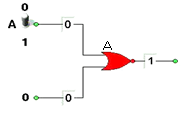
\includegraphics{figures/2.png} \caption{Προσομοίωση Πύλης \en{NOR}}\label{figureB.1}
\end{figure}

Το Σχήμα~\ref{figureB.1} απεικονίζει .................


\subsection{Περιγραφή υποσυστημάτων}
Παρακάτω δίνεται λεπτομερής περιγραφή για καθένα από τα συστήματα
που αναφέραμε. Η περιγραφή αυτή γίνεται με βάση τα διαγράμματα
ροής δεδομένων.

\subsubsection{Υποσύστημα δημιουργίας σχήματος}
Το υποσύστημα αυτό ...............
 %    \chapter{Παραδείγματα Βιβλιογραφικών Αναφορών}

\begin{center}
	\begin{tabular}{|c|c|}
    	\hline
    	\textbf{Τύπος βιβλιογραφικής πηγής} & \textbf{Αριθμός αναφοράς} \\
    	\hline\hline
    	Βιβλίο ξενόγλωσσο &  \cite{goossens93} \\
    	\hline
    	Βιβλίο ελληνικό &  \cite{greekbook} \\
    	\hline
    	Άρθρο σε επιστημονικό περιοδικό &  \cite{LiArTs13} \\
    	\hline
    	Παρουσίαση σε επιστημονικό συνέδριο &  \cite{dcis2011} \\
    	\hline
    	Ιστοσελίδα &  \cite{LaTeXProject} \\
    	\hline
    	Διπλωματική εργασία &  \cite{zoi04} \\
    	\hline
    	Πτυχιακή εργασία &  \cite{elli05} \\
    	\hline
    	Μεταπτυχιακή διπλωματική εργασία &  \cite{master04} \\
    	\hline
    	Διδακτορική διατριβή &  \cite{phd045} \\
    	\hline
    	Δίπλωμα ευρεσιτεχνίας (πατέντα) &  \cite{viswanathan2014convenient} \\
    	\hline
    	Τεχνική αναφορά &  \cite{MSU-CSE-05-29} \\
    	\hline
    \end{tabular}
\end{center}

          


 %    \chapter{Δημιουργία Ευρετηρίου}
Δείτε το περιεχόμενο του αρχείου \en{appD.tex} για τρόπους ορισμού ελληνικών και ξενόγλωσσων όρων ευρετηρίου.

% Παραδείγματα ξενόγλωσσων όρων
\indexEN{xerox} \indexEN{babel} \indexEN{anna} \indexEN{babylon}

% Παραδείγματα ελληνικών όρων (προσέξτε τη χρήση λατινικού προθέματος για τη σωστή ταξινόμηση των όρων) 
\indexGR{P@πτυχιακή} \indexGR{E@έλενα} \indexGR{E@ελένη} \indexGR{X@χρώμα} \indexGR{R@ροή} \indexGR{Z@ώριμος} \indexGR{A@άννα} 

 %    \chapter{Εισαγωγή Εικόνων}
Δείτε το περιεχόμενο του αρχείου \en{appE.tex} για τον τρόπο εισαγωγής εικόνων.

\begin{Illustration}[!h] 
	\centering
	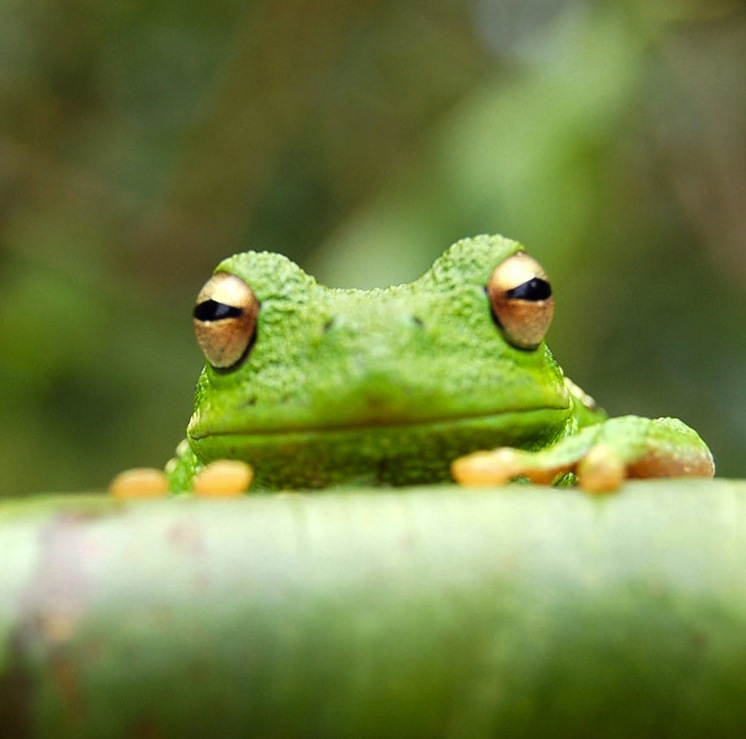
\includegraphics[width=0.5\textwidth]{figures/frog.jpg} 
	\caption{Βάτραχος}
	\label{frog_image}
\end{Illustration}
 
% Βιβλιογραφία - Αναφορές
	\bibliography{references}
% Συντομογραφίες - Αρκτικόλεξα - Ακρωνύμια
	\includeabbreviations{back_matter/abbreviations}
% Γλωσσάριο
	\includeglossary{back_matter/glossary}
%%%%%%%%%%%%%%%%%%%%%%%%%%%%%%%%%%%%%%%%%%%%%%%%%%%%
% Ευρετήριο Όρων
	\printindices
%
%%%%%%%%%%%%%%%%%%
%%%%%%%%%%%%%%%%%%

%% Δημιουργία ετικετών CD:

	\definecdlabeloffsets{0}{-0.65}{0}{0.55} % upper label x offset [cm] (default=0) /  upper label y offset [cm] (default=0) /  lower label x offset [cm] (default=0) /  lower  label y offset [cm] (default=0) -- For Q-Connect KF01579 labels use the following offset values: {0}{-0.65}{0}{0.55}

	\createcdlabel{Πρότυπο Σύστημα Ομότιμων \\ Κόμβων Βασισμένο σε Σχήματα \en{RDF}}{Κωνσταντίνος Δ. Δημητρίου}{ΟΚΤΩΒΡΙΟΣ}{2020}{8} % τίτλος διπλωματικής / όνομα συγγραφέα / μήνας / έτος / εύρος περιοχής τίτλου σε cm (προτεινόμενη τιμή: 8) 

%%σ
%% Δημιουργία εξωφύλλου θήκης CD:

	\createcdcover{Πρότυπο Σύστημα Ομότιμων \\ Κόμβων Βασισμένο σε Σχήματα \en{RDF}}{Στάμος Φ. Ευάγγελος}{ΟΚΤΩΒΡΙΟΣ}{2020}{10} % τίτλος πτυχιακής / όνομα συγγραφέα / μήνας / έτος / εύρος περιοχής τίτλου σε cm (προτεινόμενη τιμή: 10) 

%%
%
\end{document}

%%%%%%%%%%%%%%%%%%%%%%%%%%%%%%%%%%%%%%%%%%%%%%%%%%%%
